\documentclass[]{article}
\usepackage{graphicx}
\usepackage{mathtools}


%opening
\title{Appunti Social Issues in Information Society}
\author{}
\date{}



\begin{document}



\maketitle
\tableofcontents

\addcontentsline{toc}{section}{Lezione 1}
\section*{Lezione 1 - 05/11/2018}

Baricco, The Game, Introduction:

Gli umani sembrano aver disimparato tutto ciò che avevano imparato dai
loro padri, come mangiare, studiare, divertirsi. Un particolare
sconcerto era nella osservazione quotidiana dei figli: li sembrava una
retro marcia nel miglioramento della specie. Incapaci di concentrarsi,
sempre attaccati a qualche computer, si intuiva l'annuncio di qualche
crisi e l'imminenza di una apocalisse culturale. La faccenda non era
chiarissima, sicuramente c'entrava sicuramente la rivoluzione digitale e
la globalizzazione. Altri umani, molti in California, stavano cambiando
il mondo tecnicamente, senza spiegare agli umani il loro progetto, e
forse senza sapere quali conseguenze avrebbe avuto tutto ciò. Ma come
mai abbiamo accettato l'idea di una rivoluzione? Ora abbiamo tante cose
che vent'anni fa non esistevano: Wikipedia, Facebook, YouTube,\ldots{}
che occupano una buona parte del nostro tempo, così tanto che ci
chiediamo come facevamo 20 anni fa a passare il tempo. È un mondo che
non saperemo mai spiegare, è una rivoluzione di cui non sappiamo né
l'origine, né lo scopo. L'autore sente l'emozione della paura nei
confronti di tale rivoluzione.

I biologi classificano essere viventi in specie: A una specie
appartengono quelli esseri che possano riprodursi fertili. Le specie che
hanno un antenato in comune e che si sono evolute sono raggruppati in genere.
Noi siamo del genere homo specie sapiens, i generi a loro volte solo raggruppati
in famiglie. Ci siamo evoluti dagli australopitecus, da cui è uscito uomo
di Neanderthal più muscolosi dei sapiens. Da 2.5 milioni di anni a circa
10 mila anni fa, il pianeta è occupato da diversi specie di homo, negli
ultimi 10mila anni fa l'uomo è salito sulla vetta del cibo piramide,
dovuto al cervello più sviluppato, circa 70 mila anni fa si sono diffusi
da Africa orientale in medio oriente e poi in tutti il mondo ma perché i
neanderthal sono scomparsi, vi sono 2 teorie:

\begin{enumerate}
	\def\labelenumi{\arabic{enumi})}
	 
	\item
	Teoria di Fusione ( siamo l'unione di più specie)
	\item
	Teoria del Rimpiazzo ( i sapiens hanno rimpiazzato le altre)
\end{enumerate}

Qualcuno dice che probabilmente è veritiera l'unione delle due.
La più accettata è quella del rimpiazzo, i sapiens era più efficaci
come cacciatori, una organizzazione sociale migliore e tecnologicamente
avanzati rispetto ai neanderthal. E' il primo caso di genocidio mai
registrato, hanno spazzato via tutti i neanderthal. L'altra ragione è
l'invenzione del linguaggio e il pensiero astratto che sono dovute
all'evoluzione. Queste realizzazioni sono dovute a una rivoluzione della
capacità cognitiva dei sapiens.

La rivoluzione cognitiva introduce nuove capacità:

\begin{itemize}
	\item
	permette di trasmettere più volumi di informazione, che ha permesso di
	pianificare e mettere azioni più complesse, come cacciare i leoni e/o
	bisonti;
	\item
	inventare nuovi oggetti utili;
	\item
	trasmettere maggiori volumi di informazione circa le relazioni sociali
	e ciò ha permesso creazioni di gruppi più ampi e coesi, fino a 150
	persone (I neanderthal invece erano meno popolosi quindi è stato
	facile per i sapiens sterminarli);
	\item
	rasmettere un pensiero più astratto quindi circa cose che non
	esistono nella realtà, tra i quali gli spiriti tribali, nazioni,
	responsabilità, diritti e questo ebbe come conseguenza:
	
	\begin{itemize}
		 
		\item
		cooperazione di numero molto alto di estranei grazi alle credenze
		comuni;
		\item
		rapida innovazione del comportamento sociale.
	\end{itemize}
\end{itemize}

Questo aumento della capacità cognitiva può essere dovuto ad una mutazione genetica
o,secondo una teoria,il linguaggio si è sviluppato grazie ai pettegolezzi,
proponendo la visione dell'homo sapiens come un animale sociale.



I passaggi dalla preistoria a storia e infine iperstoria sono definiti
in base al ciclo di vita dell'informazione. Il ciclo è costruito in
questo modo: Informazione si: Crea/Genera $\Rightarrow$ Raccoglie $\Rightarrow$ Immagazzina $\Rightarrow$
Elabora $\Rightarrow$ Distribuisce/Trasmette $\Rightarrow$ Consuma/Utilizza $\Rightarrow$ Ricicla/Cancella $\Rightarrow$
Crea/Genera l'informazione.

Nella Preistoria, parte fondamentalmente dalla rivoluzione agricola
circa 10 mila A.C., in questa epoca non ci sono forme di ICT (intendiamo
per ICT forme di immagazzinamento/documentazione documentate), le ICT
compaiono nella storia (circa 6000 anni fa, 3000-4000 A.C.) invece il
benessere non è ancora collegato alle ICT (nel ciclo di vita
dell'informazione ci si ferma all'immagazzinamento, l'informazione non
si processa), l'iperstoria invece è dipendente dalle ICT:il 
benessere sociale-individuale dipende da come si
processa e si fa uso delle informazioni.

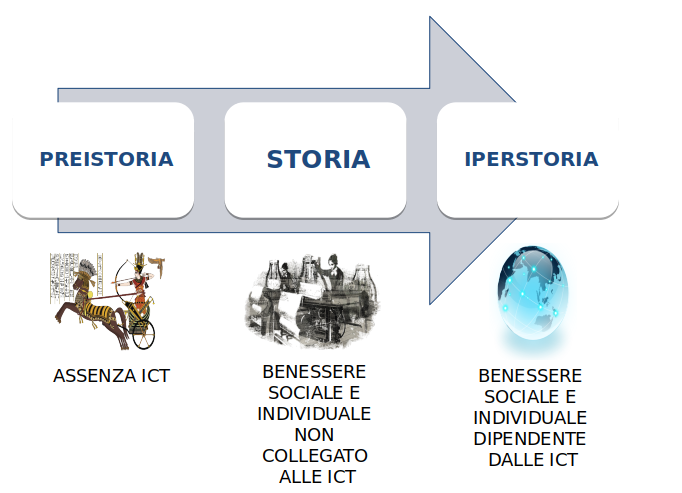
\includegraphics[scale=0.6]{image1.png}
\newline
Due tipi principali di rivoluzioni sono:

\begin{itemize}
	 
	\item
	Rivoluzioni Politiche: sono caratterizzata da violenza e rapidità che
	sono tra loro collegate, sono cambiamenti traumatici dello stato del
	mondo o dello stato del paese dovute a fenomeni profondi che hanno a
	che fare con le classi sociali e/o economici, questa violenza e
	rapidità viene mostrata nella prima metà del 1900.
	\item
	Rivoluzione Tecnologiche e Scientifiche: in se per se non violente ma
	hanno delle conseguenze che possono avvolte esserlo.
\end{itemize}

Thomas Kuhn sostiene che le rivoluzioni scientifiche mettono in crisi un
intero paradigma del mondo e finché il nuovo paradigma non si afferma,
la rivoluzione scientifica non può passare.

La rivoluzione digitale è in primo luogo una rivoluzione tecnologica. Le
rivoluzioni tecnologiche sono dovute all'invenzione di oggetti/strumenti
nuovi e ciò cambia il modo di vivere, le rivoluzioni tecnologiche
possono anche essere fantastiche ma di rado producono una rivoluzione
mentale. Una rivoluzione tecnologica può essere disruptive sulla società
o economia ma diventa mentale se modifica profondamente il modo di
pensare e i valori delle persone, vengono anche dette rivoluzione
scientifiche.

Le rivoluzione tecnologiche principali sono :

\begin{enumerate}
	\def\labelenumi{\arabic{enumi}.}
	 
	\item
	rivoluzione dell'agricoltura (decimo millennio prima dell'età moderna)
	E' una delle rivoluzione più difficile perché hanno forzato l'uomo a
	lavorare di più ma è ciò che fondato il mondo attuale;
	\item
	rivoluzione Industriale(seconda metà del diciottesimo secolo);
	\item
	rivoluzione dell'informazione(nascono tecnologie digitali, metà del
	diciannovesimo secolo).
\end{enumerate}

Rivoluzione scientifiche principali sono:

\begin{enumerate}
	\def\labelenumi{\arabic{enumi}.}
	 
	\item
	rivoluzione copernicana (La terra non è al centro) $\rightarrow$ ha avuto bisogno
	di molto tempo prima che questo paradigma passasse nella società
	dovute agli impatti sociali e religiosi che portava con se.
	\item
	rivoluzione darwiniana (l'uomo non è più al centro del mondo animale)
	$\rightarrow$ L'uomo non è non solo al centro del mondo ma manco tra gli animali
	(un'altra mazzata)
	\item
	rivoluzione freudiana (La mente umana non è trasparente a se stessa
	caratterizzata dall'inconscio e dal meccanismo del repressione)
	$\rightarrow$Un'altra mazzata perché dice che l'uomo manco capisce se stesso
	\item
	rivoluzione dell'informazione $\rightarrow$ non siamo entità isolate ma
	interconnessi che condividono con agenti biologici e artefatti tecnici
	un ambiente globale costituito dall'informazione : l'infosfera. Ha una
	caratteristica di assorbire il mondo reale e inglobarlo in un mondo
	informatico.
\end{enumerate}

La rivoluzione informatica,basata sul silicio e non più sul carbonio,
è quindi non solo rivoluzione tecnologica ma anche scientifica.

\addcontentsline{toc}{section}{Lezione 2}
\section*{Lezione 2 - 07/11/2018}

Concetto dell'Infosfera :

I fattori che accelerano la transizioni verso la società
dell'informazione sono:

\begin{enumerate}
	\def\labelenumi{\arabic{enumi}.}
	 
	\item
	legge di Moore: la tecnologia di un microcircuito raddoppia ogni 18
	mesi.
	\item
	legge di Metcalfe: se n = numero di utenti il numero massimo di
	connessione possibili è n(n-1)/2, ciò la crescita del numero di
	connessione, e di conseguenza il costo riguardante la tecnologia, è
	quadratica rispetto agli utenti.
	\item
	Forte crescita dei dispositivi connessi
	\item
	Sviluppo sinergico delle nuove tecnologie digitali (Cloud, Iot,
	Mobile)
	\item
	Crescita esponenziale dei Big Data.
\end{enumerate}

Cosa sono i Big Data :

\begin{itemize}
	 
	\item
	Secondo IDC: Una nuova generazioni di tecnologie e architetture
	disegnate per estrarre il valore economico da grandi volumi e varietà
	di dati, utilizzando grandi velocità, gestione e analisi. I 5V sono:
	Velocità, Volume, Varietà, Variabilità e Veridicità.
	\item
	Secondo NIST : I Big Data si riferiscono all'inabilità delle
	architetture tradizionali per la gestione dei dati, a gestire
	efficacemente nuovi dataset. Le caratteristiche dei Big Data sono :
	Volume, Velocità, Varietà e/o Variabilità. I Big Data consistono nella
	distribuzione orizzontale e indipendente dei dati per ottenere la
	scalabilità richiesta per una gestione dei database estensivi. 
\end{itemize}


I Big Data sono diversi perché hanno alti Volumi e sono non strutturati
devono essere memorizzati e processati rapidamente quindi richiedono
nuove architetture, modi di processare e visualizzare questi dati.
Bisogna poter scalare sia in verticale (aumento di potenza),
sia in orizzontale con l'utilizzo di risorse distribuite.

I benefici dei Big Data sono:

\begin{enumerate}
	\def\labelenumi{\arabic{enumi}.}
	 
	\item
	Identificare clienti a più alto potenziale, per l'opportunità di
	cross-selling e l'efficacia delle campagne e dei canali. (Ho un
	(crica) ROI -- Return on Investement del circa 41-56\%).
	\item
	Identificare i bisogni dei clienti (ROI -- 40-48\%)
	\item
	Identificare i clienti a rischio e analizzarne il comportamento (ROI
	-- 54\%)
	\item
	Monitorare la qualità e quantità (ottimizzata) dei prodotti necessari
	(50-70\%)
	\item
	Misurare il rischio, pianificazione, budgeting e forecasting (69\%)
	\item
	Migliorare la retention delle risorse e l'efficacia dei recruting
	(48\%)
\end{enumerate}

Il loro maggior utilizzo è nel :

\begin{itemize}
	 
	\item
	Social Intelligence -- Sentiment Analysis, Social Customer Care
	\item
	Predictive Analytics -- Elasticità del prezzo, Riduzione delle frodi
	\item
	Segmentation Insights -- Analisi Funnel, Pattern nei comportamenti
	\item
	Mobile Analytics -- Pubblicità mirate, Analisi Geo-Spaziali.
\end{itemize}

Dalla legge di Moore la potenza per gestire i dati aumenta
esponenzialmente ma i data crescono in una maniera anch'essa
esponenziale anzi più veloce della legge di Moore, quindi i vecchi
modelli per gestire i dati non basterà più ma allo stesso momento avremo
un preprocessing power molto più forte.

I Tre ordini delle tecnologie secondo Floridi sono:

Per il suggeritore intendiamo il motivo che mi costringe a creare una
tecnologia, ad esempio il la pioggia suggerisce la creazioni
dell'ombrello. E la tecnologia è quello che si piazza tra l'utente e il
suggeritore stesso. E secondo Floridi non vi sarà una tecnologia del 4$^o$
ordine ma solo tecnologie che connettono varie tecnologie del 3$^o$ ordine.
Nel secondo ordine il suggeritore è un'altra tecnologia (es vite-cacciavite).
Nel terzo l'uomo ha il controllo del processo ma non vi è in esso (internet
of things).

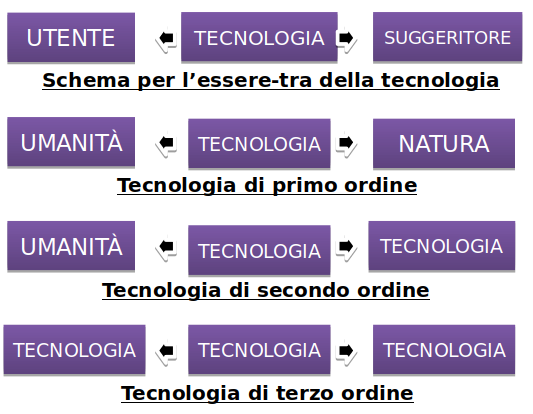
\includegraphics[scale=0.6]{image2.png}

Lo ZettaByte corrisponde a 10$^{21}$ byte nel 2011 abbiamo raggiunto 1
ZettaByte e nel 2015 siamo arrivati a 8 ZettaByte, ma la metà dei dati è
inutile ma non sappiamo quale metà è quella inutile. L'Età dello
ZettaByte può essere interpretata come il momento di transizioni tra i
Big Data ciechi e quelli dotati di vista, nel senso che riesco a dare un
senso a questi dati (trovo un pattern).

Legge di Kryder : la densità di immagazzinamento degli HD cresce più
velocemente della legge di Moore, ma il mondo produce molti più dati di
quelli che si possono immagazzinare.

Legge di Nielsen : la velocità di una rete per utenti domestici cresce
del 50\% all'anno raddoppiando ogni 21 mesi(\textless{} legge di Moore).

I colli di bottiglia che si pongono contro l'innovazione digitale sono:

\begin{itemize}
	 
	\item
	Memoria
	\item
	Connettività
	\item
	Mancanza di standard condivisi è un tema di grande importanza,si 
	tratta di un primitivismo tecnologico infatti
	spesso dei dati non possono essere visualizzati dai sistemi diversi da
	quelli che gli ha prodotti e ciò rallenta la nostra crescita
	tecnologica. 
	\item
	Il dislivello tra l'innovazione tecnologica e i tempi di adattamento
	delle organizzazioni. DESI (Digital Economy and Society Index) è
	l'indice che mostra il livello di innovazione digitale dei paesi
	europei.
	\item
	L'albero della conoscenza e lo sviluppo asincrono -- La metafora è
	quella della società dell'informazione come un albero dove i rami sono
	caotici ma le radici concettuali, etiche e culturali stentate.
\end{itemize}

La quarta rivoluzione è una rivoluzione dell'informazione: non siamo
delle entità isolate ma INFORG, Organismi Informazionali Interconnessi,
che condividono un ambiente globale costituito da informazione:
l'infosfera.

La Sfida della rivoluzione dell'informazione è affermare un nuovo
paradigma dell'uomo come animale informazionale al fianco di altri,
inserito all'interno dell'infosfera.

L'informazione deve essere considerato un bene di consumo, è un bene non
rivale : se chiunque ha accesso ai dati può servire per migliorare in
generale la situazione. Tende ad essere non esclusiva cioè più
facilmente condivisa e rivelata e ha un costo marginale che tende ad
essere trascurabile. Quindi possiamo considerala come un bene pubblico.

Il bitcoin ha introdotto un concetto di scarsità digitale, definendo
come finito il mondo del bitcoin ha introdotto un elemento che prima di
allora non esisteva.

Gli impatti sulla vita sociale ed economica sono notevoli: Il diritto
d'uso degli oggetti diventa tanto importante quanto il diritto di
proprietà e il diritto di proprietà diviene sempre meno rivelante oggi
ad es. Uno non vuole una macchina perché ha il car sharing oppure Uber,
mentre cresce il diritto d'uso di oggetti. I beni virtuali, come il
software, vengono considerati come investimento in conto capitale e non
come spese correnti.

Le definizioni dell'INFOSFERA :

\begin{itemize}
	 
	\item
	Def A : a livello minimo, l'infosfera indica intero ambiente
	informazione costituito da tutti gli enti informazionali e loro
	proprietà,processi e reciproche iterazioni.
	In questo caso si pensa ancora ad un dualismo mondo informazionale
	e mondo analogico.
	\item
	Def b : A livello massimo, l'infosfera è un concetto che può essere
	utilizzato come sinonimo di realtà laddove interpretiamo quest'ultimo
	in termini informazionali. Concezione di realtà monistica.
\end{itemize}

Le proprietà dell'Infosfera:

\begin{itemize}
	 
	\item
	Le ICT creano un nuovo ambiente informazionale dove le future
	generazioni trascorreranno la maggior parte del tempo.
	\item
	L'infosfera sta riassorbendo l'Habitat ``Naturale''
	\item
	Stiamo passando passando da una metafisica materialistica a
	informazionale.
	\item
	La soglia tra il mondo analogico, offline, di carbonio e il mondo
	digitale, online, di silicio tende a sparire.
	\item
	Il digitale si sta diffondendo nell'analogico e si sta confondendo con
	esso.
	\item
	L'infosfera tende ad assorbire ogni altro spazio e il mondo offline è
	destinato a diventare totalmente iterativo grazie all'infosfera.
	\item
	l'effetto sull'ambiente quotidiano: vivere ``Onlife'' nell'infosfera
	sempre più sincronizzata, de-localizzata e correlata.
\end{itemize}

Quindi noi dovremo lavorare a un ecologia dell'infosfera infatti:

\begin{itemize}
	 
	\item
	Il digitale divide e rischia di generare nuove forme di
	discriminazione tra chi è digitale e chi non lo è.
	\item
	si creerà nuovo divario tra società storiche e iperstoriche(per loro
	l'informazione è un bene)
	\item
	Ridisegnerà la mappa della società mondiale
	\item
	La nuova ecologia è necessaria per evitare le baraccopoli digitali.
\end{itemize}

Per fare questo bisogna essere in grado di essere una gamma di
applicazioni che:

\begin{itemize}
	 
	\item
	Migliorano: sono interfacce volte a consentire l'applicazione dello
	strumento al corpo dell'utente in modo ergonomico(impugnature,
	interruttori).
	\item
	Aumentano: i dati e i pannelli di controllo delle tecnologie che
	aumentano sono interfacce tra ambienti diversi: l'ambiente esterno
	dell'utente umano e l'ambiente della tecnologia.
	\item
	Apportano trasformazioni radicali: Le ICT modificano l'essenza del
	nostro mondo perché creano e ricostruiscono realtà che l'utente è in
	grado di abitare. Le loro interfacce sono delle porte d'ingresso per
	l'utente nell'infosfera.
\end{itemize}

Le tecnologie ICT stanno riontologizzando il mondo: ad esempio con mouse
e touch screen.
\addcontentsline{toc}{section}{Lezione 3}
\section*{Lezione 3 - 12/11/2018}

I social stanno cambiando le nostre identità personali, e questo ci
porta a delle domande e a spiegarci la loro distinzione:

\begin{enumerate}
	\def\labelenumi{\arabic{enumi}.}
	 
	\item
	Chi siamo? (la nostra identità personale)
	\item
	Chi pensiamo di essere? (la nostra concezione del se)
	\item
	Cosa pensano gli altri su cosa siamo? (la nostra identità sociale)
\end{enumerate}

La nostra generazione è inconsapevoli di sé, e lavoriamo in tutti i modi
per costruire la mia immagine social in base a quello che gli altri
pensano e su questo siamo iperconsapevoli.

Il risultato è che l'internet è la proiezione di chi vorremo essere.
Il nostro se sociale influisce su ciò che siamo veramente,dalla 
condizione sociale passiamo ad alterare la nostra identità.
Basta guardare la polarità che si è formata nell'internet ad esempio nel
caso delle elezioni.

La domanda è chi siamo noi e che cosa diventiamo dopo che siamo stati
abbastanza tempo nell'infosfera? Il paradosso di Theseus' Ship, continuo
a cambiare i pezzi quando la nave marcisce un po' alla fine la nave era
identica a quella iniziale ma non c'era neanche un pezzo originale.

L'interfaccia è molto importante per rispondere a certe domande ad
esempio, nel caso di un ospedale diventato scuola è diverso come
interfaccia dell'utilità mentre è la stessa come posizione.

Per rispondere a tale domanda partiamo con un Primo approccio:

\begin{itemize}
	 
	\item
	Descartes: ``Cogito ergo sum res cogitans'', io penso quindi io sono.
	Le mie idee sono chiare e distinte.
	\item
	John Locke: L' identità è data dall'unità della tua coscienza e dalla
	continuità della memoria.
\end{itemize}

Secondo approccio:

\begin{itemize}
	 
	\item
	Teoria narrativa del se: l'identità è una storia(auto/socio - biografia).
\end{itemize}

Ma ad esempio nel caso di pazienti di Alzheimer perdendo spesso
rapidamente la memoria perdono anche la loro identità? Secondo il primo
approccio io perdo di essere me stesso, ma il secondo no.

Il self è dunque un sistema informazione complesso, costituito da
attività coscienti, memorie o narrative, noi siamo la nostra
informazione. E le ICT sono potenti tecnologie di sé.

Concetti informazionali di sé:

\begin{itemize}
	\item
	una visione dualistica della relazione tra il corpo e la mente
	\item
	una forma di monismo basato sullo stato: materiale contro immateriale
	come differenti stati dell'informazione (una metafisica informazione).
	
	Sembra essere tornato alle prime forme della filosofia si basavano
	proprio sul rapporto tra io e il mondo.
\end{itemize}

Facciamo un paio di esempi:

1) Informazioni riguardanti e-health come una colonna per le cure
mediche nel futuro:

\begin{itemize}
	 
	\item
	Il corpo trasparente consiste nel:
\end{itemize}

\begin{itemize}
	 
	\item
	per prevenire e gestire malattie in maniera non invasiva.
	\item
	Per garantire il benessere (Apple Watch)
\end{itemize}

\begin{itemize}
	\item
	Il corpo condiviso:
	
	\begin{itemize}
		 
		\item
		Il mio corpo può essere visto come un tipo di corpo
		\item
		spostando quindi la concezione dalle mie condizioni alle condizioni
		che condivido con altri.
	\end{itemize}
\end{itemize}

2) I 3 trendi principali riguardanti l'e-health.

\begin{enumerate}
	\def\labelenumi{\arabic{enumi}.}
	 
	\item
	Democratizzazione di informazioni sulla salute, quindi la sua
	diffusione nel pubblico.
	\item
	Disponibilità e aumento di dati generati dall'utente riguardante la salute.
	\item
	Socializzazione delle condizioni di salute.
\end{enumerate}

3) e-education: ma sono sinonimi essere civilizzati, acculturato ed
educato? No, infatti

\begin{itemize}
	 
	\item
	Essere civilizzati o acculturati è un fattore locale, mentre educati è
	un più particolare.
	\item
	Nell'infosfera essere educati è un fattore che si sta velocemente
	de-localizzando e uniforme, in realtà già dalla fine del 1900.
	\item
	Educazione è una trasmissione di conoscenze e come come essa può
	essere aumentata e non più riservata solo a una classe di élite.
	\item
	ICT permettono di personalizzare l'esperienza educativa come mai visto
	prima. Ad esempio i Massive Open Online Courses sull'internet.
\end{itemize}

L'information society è una neo società che usa come materia primaria
l'informazione e ne produce come prodotto finale sempre l'informazione
che noi consumiamo. In tale società dobbiamo mettere più enfasi sulla
conoscenza del fare e non come nella vecchia società dove esisteva solo
l'episteme (scienza e sapere quella) contro techne (tecnologia e sapere
come).
\addcontentsline{toc}{section}{Lezione 4}
\section*{Lezione 4 - 03/12/2018}

Perché nella ICT la privacy diventa la domanda più importante? E che
cos'è la privacy dopo la quarta rivoluzione?

La privacy è una funzione della frizione informazionale, che è la
resistenza che si oppone alla diffusione libera dell'informazione. Data
un po' di informazione personale, più è bassa la frizione
informazionale, maggiore è l'accessibilità alle informazioni personali
fra gli agenti all'interno della regione. Più è piccolo il gap
informazionale minore è il livello di privacy che ci si può aspettare.

Nelle prime urbanizzazione, il livello di privacy è aumentato
notevolmente (nelle zone rurali tutti sanno tutto di tutti). Quindi ciò
che consente alle società lo sviluppo della privacy è l'anonimato. Ma
nella società digitale l'anonimato non può essere garantito totalmente.
Con il passare delle generazioni cambiano il concetto di ciò che
vorrebbero tenere nascosto, ciò che sono oggetti della privacy.

Mentre le vecchie ICTs (TV, radio) riducono la frizione informazionale,
le nuove ICT funzionano da entrambe le parti, infatti vi sono due
categorie di tecnologie: PET (Privacy Enhancing Tecnology) che
incoraggiano l'equalità e migliorano sia la quantità che qualità dei
prodotti e PIT (Privacy Intrudincg Tecnologies) da cui nasce anche il
concetto della GDPR.

Dopo 4a rivoluzione consideriamo ciascun individuo costituito dalla sua
informazione, quindi la privacy è la natura dell'essere nella società
digitale (la sua identità), la rottura della privacy è la aggressione
contro la mia persona. Le ICTs possono sia erodere che migliorare la mia
privacy. C'è una distinzione di personalità tra social e realtà. C'è il
problema del aumento del furto di identità come uno dei principali
attacchi nella società digitale.

Vi sono diversi problemi etici che sorgono dai social network:

\begin{itemize}
	 
	\item
	Incitazione all'anoressia o altre atti sbagliati.
	\item
	Il caso di Target, quello della ragazza incinta in USA e Target è un
	supermercato.
	\item
	BlueWhale
\end{itemize}

Vediamo la politica nel mondo digitale:

Nel 1648 con la pace di Westfalia che finì la guerra dei 30 anni e la
guerra dei 80 anni, come conseguenza nascono i stati nazionali come li
conosciamo noi oggi (recentemente è nata la crisi dei stati nazionali),
gli stati sono agenti indipendenti, che giocano il ruolo istituzionale
in un sistema di relazioni internazionali, caratterizzati da:

\begin{itemize}
	 
	\item
	sovranità -- diritti della autodeterminare la propria politica.
	\item
	ugualità dal punto di vista del diritto fra i vari stati nazionali
	\item
	astenzione dall'intervento negli affari interni di altri paesi.
\end{itemize}

I stati nazionali agiscono come agenti indipendenti che possono
aumentare tasse entro i loro confini, contrattare debiti come entità
legali e difendere i propri confini.

Montesquieu suggerì la divisione classica della politica dello stato:
Legislazione , esecutivo e giudiziario. Lo stato è un multi agente si
organizza come una rete di questi tre mondi. ICT per uno stato nazionale
è uno strumento per esercitare la sua forza legale, potere politico e
controllo sociale.

L'evoluzione dallo stato nazionale all'inizio della trasformazione
profonda avviene con ``Washington Consensus'' nel 1989, è un insieme di
10 raccomandazioni che rappresentano la strategia standard per una
stabilizzazione macroeconomica dei paesi con lo stato durante una crisi
e viene applicata da istituzione come IMF, World Bank. LeICT si spostano
da una forma di governo centralizzato a una forma di governo distribuito
e di coordinamento internazionale per gestire crisi di grande
complessità internazionale.

Con la Bretten Woods conference nel 1944 nasce la crisi dello stato
nazionale introdotto del 1648 introducendo nuovi concetti come World
Bank, World trade, IMF (International monetary fund) che regolano i
problemi internazionali fra i vari stati nazionali.

Le 4 conseguenze di ICS, che spiegano il passaggio da una situazione
storica a una situazione iperstorica:

\begin{enumerate}
	\def\labelenumi{\arabic{enumi})}
	 
	\item
	Potere: ICT democratizzano l'esercizio del potere, e danno il potere a
	una serie di agenti non statuali (es. le multinazionali). E questo
	genera una nuova tensione fra potere informazionale e potere fisico.
	\item
	Geografia: Le ICT de-localizzano l'esperienza umana, rendendo
	irrilevante i confini, creando regione dove prevale onlife, generando
	nuove tensioni tra la geopolitica globale e lo stato.
	\item
	Organizzazione: Le ICT fluidificano la topologia della politica,
	generando nuove tensioni fra gli stati, trasformandoli in sistemi
	multi agenti e una varietà di multi-agenti non-stati. Ad esempio ISIS.
	\item
	Democrazia: Le ICT fanno nascere forme di democrazia diretta come
	opzione complementare ma spesso la democrazia diretta si trasforma
	spesso in una democrazia condotta dai mass-media. Questo spesso sporca
	la democrazia.
\end{enumerate}

L'internet sta modificando la comunicazione politica, stanno
jeopardizing la democrazia? Permettono la profilazione economica e
politica dei propri utenti. Allo stesso momento diventano necessari per
la politica stessa: sicuramente ``Non potete vincere le elezione stando
su internet, ma perderete sicuramente se non ci siete.''

Dal conflitto storici che erano armati (ad esempio quando la politica
fallisce) si passa ai cyberwar e conflitti con metodi digitale
nell'iperstoria, 4 sono le modifiche principali:

\begin{enumerate}
	\def\labelenumi{\arabic{enumi})}
	 
	\item
	Le ICT hanno progressivamente rivoluzionato le comunicazioni, rendendo
	possibile nuove modalità operative.
	\item
	Le ICT e i Big Data sono delle armi, analizzando la grande quantità
	dei dati permette all'intelligenza militare di prendere azioni
	rapidamente.
	\item
	Le battaglie sono combattute con dispositivi ICT in tempo reale
	(satellite, sensori di battaglie, robot).
	\item
	La dipendenza sulle ICT avanzati hanno condotto a attacchi cyber
	strategici, aumentando il potenziale distruttivo degli attacchi.
\end{enumerate}

Il terrorismo suicida si è trasformato in cyberwar nella iperstoria e
gli attacchi cyber possono essere intrapresi sia da nazioni, reti oppure
piccoli gruppi piccoli e ciò facilita I conflitti asimmetrici. Ponendo
quindi vari problemi etici : 1) diritti, 2) Rischi, 3) Responsabilità.
In poche parole, l'information war ha bisogno di una nuova etica
informazionale.

Il costo del digitale sull'ambiente:

I geologisti sembrano essere d'accordo sui impatti significativi
sull'ecosistema debba essere riconosciuto adottando una nuovo epoca
``Anthropocene'' che fino ad ora non esiste. La nuova era ha dei costi
ambientali alto, se non insostenibile. L'infosfera sta jeopardizzando la
biosfera, quindi dobbiamo essere attenti alle implicazioni della
tecnologia sulla natura. Alcuni esempi sono: il versamento del petrolio
nell'ambiente marino, l'esplosione di Chernobyl ecc. per questo motivo
un numero di sistemi legali e tecnologie per la sicurezza si stanno
sviluppando e costituiscono i cosi detti metatecnologie. Si può agire in
diversi modi alcuno sono:

\begin{itemize}
	 
	\item
	La prevenzione: Un po' troppo radicale, quando si banna una tecnologia
	completa, può avere effetti devastanti sui piano di crescita in corso.
	(ban nucleare in Italia)
	\item
	Limitazione e riparazione: Le prevenzione relative come misura che
	permette a una tecnologia di svilupparsi, ma cerca di prevenire o
	almeno limitare i suoi rischi ma non sempre efficaci (tsunami nella
	centrale nucleare di Fukushima)
	\item
	Compensazione: ci sono modi per gestire i costi prima (con
	l'assicurazione) o dopo (compensazione) quando una tecnologia
	fallisce. Deve essere ben calibrato. Ad esempio, dopo un versamento di
	petrolio in Alaska, la compagnia fu multata solo di 75 milioni \$ ma
	il danno ammontò a 2.3 billioni \$.
\end{itemize}

Le ICT stanno potrebbero giocare un ruolo molto importante nella crisi
ambientale ma sono consumano tanta elettricità, i ZettaByte richiedono
ZettaWatts. E' stimato che le emissioni dovute alle ICT aumenteranno di
circa 6\% all'anno. Quindi abbiamo che le ICT sono sia potenziali energy
savers che inquinanti. Quello che speriamo è che il beneficio delle ICT
migliorino l'ambiente più del danno che fanno, e che ci sia abbastanza
tempo per poter recuperare il danno già fatto.
\addcontentsline{toc}{section}{Lezione 5}
\section*{Lezione 5 - 05/12/2018}

Il mondo sta cambiando dall'analogico al digitale, inoltre
l'intelligenza artificiale sono macchine che fanno molte cose ma non
sono intelligenti, è lì il problema. Inoltre non c'è più la differenza
tra offline e online, è un mix di tutte e due, infatti si chiama
infosfera laddove viviamo oggi.

5 sfide per sfruttare queste possibilità:

\begin{enumerate}
	\def\labelenumi{\arabic{enumi})}
	 
	\item
	Vulnerabilità: Il digitale fa pasticcio per tutti, piccoli grandi,
	potenti o meno. Lo possiamo aggiustare usando sempre il digitale, in
	po' come l'antivirus.
	\item
	Complessità: un sistema ha tanti rapporti che se cambi una cosa qua
	cambierà qualcosa da qualche altra parte senza che io possa
	prevederlo. 
	\item
	Sostenibile: dobbiamo essere amichevoli nei confronti del mondo perché
	altrimenti se non c'è un pianeta dove abitare cosa facciamo di questo
	sviluppo tecnologico. 
	\item
	Lavoro: Quello che è importante per noi non è il lavoro bensì il
	salario. Ma le AI saranno un aiuto per il nostro lavoro per renderlo
	più efficiente, ma non possono sostituire l'umano.
	\item
	Autonomia: E' molto importante perché i gadget ci dicono cosa ci piace
	o meno.
\end{enumerate}

Non si può vincere solo con le regole come GDPR (servono anche loro),
bisogna avere una strategia vincente che è l'etica.

Qual'è la differenza tra data e informazione? Sia X diverso da Y, dove X
e Y sono due variabili non interpretate e la relazione di essere
distinti sono lasciate per ulteriore interpretazione. Quindi il dato è
assenza di uniformità, la definizione può essere applicata in tre modi:

\begin{itemize}
	 
	\item
	I dati possono essere la mancanza dell'uniformità nel mondo reale.
	\item
	I dati possono essere la mancanza dell'uniformità tra due stati fisici
	del sistema.
	\item
	I dati possono essere la mancanza dell'uniformità tra due simboli.
\end{itemize}

Definizione generale dell'informazione: $sigma$ è un l'istanza
dell'informazione, compreso come contenuto semantico, se e solo se:

\begin{itemize}
	 
	\item
	è costituito da n dati, con n\textgreater{}0.
	\item
	i dati sono ben formati, cioè sono messi insieme nel modo corretto,
	secondo regole scelte dal sistema, codice o linguaggio.
	\item
	I dati ben formati hanno un significato.
\end{itemize}

Secondo una scuola (di Floridi), la nostra tecnologia corrente non è
capace di processare alcun tipo di informazione significativa priva di
semantica, cioè il significato e l'interpretazione dei dati è
manipolata.

Il problema di inquadramento: come un agente situato può rappresentare
un cambiamento dell'ambiente e interagire con esso. I computer sono
puramente macchine sintattiche, che possono processare dati non
interpretati secondo delle regole(sintassi), incapaci di apprezzare la
caratteristica semantica (significato) delle entità coinvolte e delle
loro relazioni.

Qui abbiamo il problema principale della robotica: In che modo i dati
acquistano il loro significato.

I rischi dei problemi diventano insormontabili quando la loro soluzione
richiede manipolazione dei dati. Secondo questa scuola, siamo noi agenti
intelligenti a eccellere nel processare significati, ma non sappiamo
esattamente come. Secondo questo pensiero c'è una soglia semantica tra
noi e le nostre macchine che non sappiamo come recuperare.

Questo ha portato a un due visioni di A.I.:

\begin{itemize}
	 
	\item
	Intelligenza Forte contro debole, A.I. leggero contro forte
	\item
	Ingegneristico contro cognitivo
	\item
	Produttivo contro ri-produttivo
\end{itemize}

Cercando si superare questa semantica, AI ha sviluppato nuove aree di
ricerca, dette le nuove AI, tra cui NN, Bayesian system, ML, robot
situati etc.

Una visione alternativa è quello di Ray Kurzweil che è quella della
singolarità. È una ipotesi che l'invenzione di AI, accelererà
bruscamente la crescita tecnologica che cambierà profondamente la
civilizzazione come la conosciamo. Secondo tale ipotesi le AI entreranno
in un ciclo di auto miglioramento che risulterà in una intelligenza
superiore a quella umana. La data predetta è 2045.

An Ethical Framework for a Good AI Society based on AI4 People.

La società AI porta con sé le opportunità e i rischi, in particolare 4
opportunità principali a cui corrispondono 4 rischi del cattivo uso, del
sovrauso e del poco uso di esso:

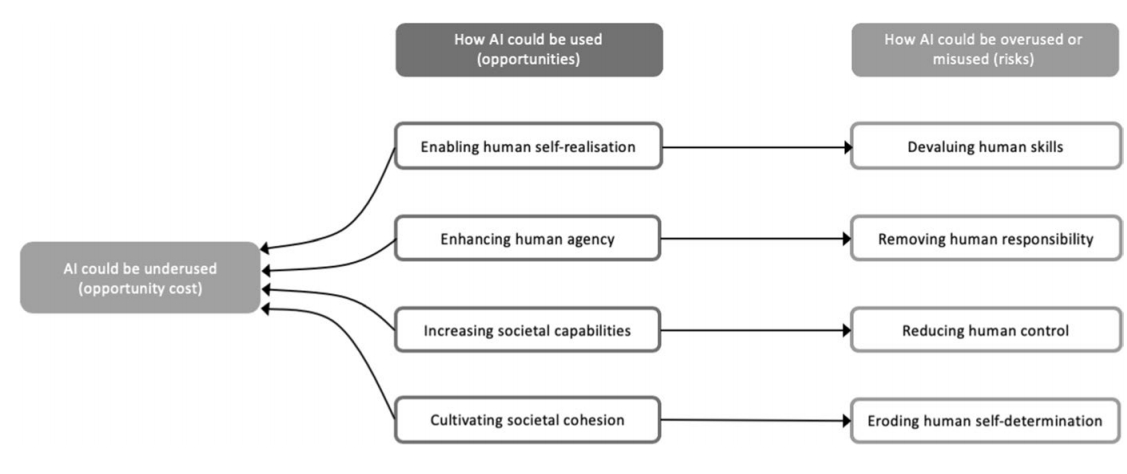
\includegraphics[scale=0.3]{image3.png}

Le 4 opportunità offerte da AI sono:

\begin{itemize}
	\item
	Chi possiamo diventare: Aumentare la realizzazioni propria senza
	devalutare abilità umane. Potremo avere più tempo libero per noi
	stessi.
	
	\begin{itemize}
		 
		\item
		Rischi: Questo potrebbe generare un digital skill mismatch e
		ridondanza. Potrebbe favorire la distribuzione non equa di costi e
		benefici che ne sono il risultato. 
	\end{itemize}
	\item
	Che cosa possiamo fare: Aumentare agenzia umana, senza rimuovere la
	responsabilità umana, dobbiamo pensare quest'opportunità come mezzo
	per fare di più e più velocemente grazie alle AI ma la responsabilità
	rimane essenziale.
	
	\begin{itemize}
		 
		\item
		Rischi: Assenza di responsabilità, un framework socio-politico
		sbagliato e la creazione di una mentalità blackbox.
	\end{itemize}
\end{itemize}

Se sviluppato bene moltiplica le opportunità e le possibilità per gli
umani.

\begin{itemize}
	\item
	Che cosa possiamo ottenere: Le capacità sociali migliorate senza
	ridurre il controllo umano.
	
	\begin{itemize}
		 
		\item
		Le AI offrono tanti possibilità di migliorare la nostra società ad
		esempio: nel caso di medicina, trasportazione e logistica, oppure
		rinventare la società radicalmente aumentando ciò che gli umani
		sono.
		\item
		Rischi: Non essere dentro o sopra il loop, riduce la nostra abilità
		di monitorare il funzionamento di questi sistemi.
		\item
		Quindi dobbiamo tenere sotto controllo gli sviluppi più grandi e i
		loro effetti.
	\end{itemize}
	\item
	Come possiamo interagire: Coltivare la coesione umana senza erodere
	l'autodeterminazione umana, con i problemi globali sta aumentando il
	senso di coordinazione complessiva, che può essere trattata solo se
	tutti i stakeholder cooperino per risolvere i problemi. Le AI dono i
	loro algoritmi basati sui dati possono aiutare tanto in questo ambito,
	ad esempio per il cambiamento climatico. La potenza predittiva delle
	AI deve essere al servizio dell'umanità e non toccare la dignità
	umana.
\end{itemize}

Ci sono vantaggio doppio per l'approccio etico alle AI:

\begin{itemize}
	 
	\item
	L'etica permette alle organizzazioni di prendere vantaggi che la AI
	crea, permettendo così di avere nuove opportunità che sono socialmente
	accettate o preferite.
	\item
	Ma evita anche errori costosi, prevenendo o mitigando azioni che
	potrebbero diventare socialmente inaccettabili quindi rigettate.
\end{itemize}

I 5 principi proposti da cui 4 dalla bioetica sono: 1) La beneficenza:
promuovere il benessere, preservare la dignità e sostenere il pianeta.
2) Non malificenza: Privacy, sicurezza ed prevenire altri danni. 3)
Autonomia: Il potere di decidere o decidere di decidere. 4) Giustizia:
Promuovere la prosperità e preservare la solidarietà. 5) Trasparenza o
Esplicabilità: Avvia gli altri principi attraverso l'intelligibilità e
applicabilità, in modo che il sistema sia trasparente a noi.
\addcontentsline{toc}{section}{Lezione 6}
\section*{Lezione 6 - 10/12/2018}

Gli impatti della tecnologia digitale sui modelli del business che hanno
caratterizzato il periodo fino al 2015 sono per esempio Mobile internet,
Big Data, tecnologia cloud, crowd sourcing, urbanizzazione rapida,
lavoro più flessibile, cambiamento climatico, volatilità geo-politica,
sviluppo della classe media, longevità della vita. Dal 2015 al 2017
invece ci si è concentrati più sull'aspetto etico con il potere alle
donne, privacy, nuove etiche e stampanti 3D. Dal 2018 in poi abbiamo la
robotica, trasporti automatici, AI, biotecnologie.

Il periodo di payback nel mondo della robotica sta scendendo, e ciò
determina o un problema o un opportunità, se posso pagare un robot 1
euro all'ora allora non assumerò più umani, ma per l'imprenditore è un
opportunità. Questo è un problema più grave nei paesi in fase di
sviluppo e se andiamo a vedere la distruption nei vari settori del
lavoro abbiamo che i settori più colpiti sono: Servizi finanziaria,
infrastrutture e mobilità (macchine auto pilote), il settore di ICT: i
settori come quelli di ufficio e amministrazione, produzione e
manufacturing, costruzione ed estrazione, arte sport, media, legali sono
a impatto negativo, mentre i settori come business, gestione,
informatica, matematica, architettura e ingegneria avranno un impatto
positivo.

Abbiamo che le occupazioni ristrutturate (le competenze rimangono
sicure, ma la forma del valore è mutevole) come nel caso di insegnante
accademico, fotografo, mentre le occupazioni messe fuori mercato (le
abilità sono considerate obsolete) sono quelle del casellante,
bibliotecario. Le occupazioni riqualificate (di cui le competenze sono
standardizzate ma ai consumatori piace comunque il modo in cui viene
fornito il valore) sono quelle del muratore, cameriere al fast-food
mentre le occupazioni durevoli sono quelle del infermiere, idraulico,
elettricista.

Il passaggio dall'analogico al digitale ha dei vantaggi e svantaggi:

Vantaggi:

\begin{itemize}
	 
	\item
	Più ricchezza viene creata con poco lavoro
\end{itemize}

Svantaggi:

\begin{itemize}
	 
	\item
	Perdita di lavoro, caso di Kodak che viene sostituita da Instagram e
	miglia di operai perdono il lavoro e devono cercare altri modi per
	sostenersi.
	\item
	La ricchezza però è in mano ai pochi, e il divario economico sta
	aumentando sempre di più.
\end{itemize}

Coloro che sono riusciti a cogliere quest'opportunità e accumulare i
giusti assetti:

\begin{itemize}
	 
	\item
	Capitali non umani: assetti finanziari, equipaggiamento, proprietà
	intellettuali
	\item
	Capitali umani: educazione, esperienza e abilità.
\end{itemize}

Quindi non è vero che questo sviluppo aiuterà tutti, anzi recentemente
le tecnologie digitali vengono usate anche per i lavori di tutti i
giorni sostituendo il lavoro di chi lo faceva prima, ma le tecnologie
come i big data aumentano la richiesta del valore e dei skill.

Complessivamente si riduce la richiesta per il lavori con meno skill,
mentre aumentano quello che richiedono più skill.

Un'altra questione è l'opinione pubblica pessimista sul futuro
nonostante il GPD mondiale non è mai stato più alto di ora, né
l'innovazione tecnologica così rapida.

Un altro punto da notare è che nonostante l'occupazione stia iniziando a
scendere in generale la produttività continua ad aumentare.

A questo problema la proposta di Bill Gates è quella di tassare i
robots, questa proposta ha suscitato molte polemiche, tra cui quella di
Maffè che la definisce una idiozia economica perché ridurebbe
l'efficienza produttiva e crede che bisogna affrontarla con il Welfare e
impiegamento. Elon Musk propone una redditto universale, mentre
Bentivogli dice di detassare il lavoro umano e introdurre il diritto
soggettivo alla formazione per ridurre il gap di competenze.

Le macchine sono un organizzazione visibile delle tecniche, Marx nella
storia economica distingue tra il periodo di manifattura (basato sul
lavoro manuale) e il periodo dell'industria moderna (basato sui
macchinari), nel pensiero di Marx le macchine assorbono il lavoro. Nel
nostro periodo abbiamo i robot, internet e AI e il software è
l'organizzazione invisibile delle macchine e se alcuni il software sta
mangiando il nostro mondo. Il Software rappresenta il rischio
dell'erosione economica e organizzazione in tante professioni
intellettuali. La didattica tradizionale nel digitale sta diventando
data scalabile e condivisibile (ML, AI). Il software spiazza il capitale
finanziario (Uber, Airbnb) dove la competitività avviene dalla gestione
del canale e non solo dalla qualità del servizio.

Le tecnologie digitali riducono l'asimmetria tra domanda e offerta
perché ci porta tutti quanti allo stesso piano, ma riducono anche le
asimmetrie organizzative, quindi la differenza nei termini di capitale
organizzativo fra le aziende, ad esempio se ci sono 2 aziende
competitive con due supply chain diverse, appena le incorporo in un
unica piattaforma digitale, questa competitività svanisce.

Il risultato di tutto questo è la polarizzazione del lavoro: la
creatività viene ben pagata mentre le nicchie frammentate marginali
abbassa la loro paga, es. Data Scientist vs Badante.

Questa crisi del welfare può essere affrontata redistribuendo il valore
generato dai dati, questo tema va oltre la tassazione sui profitti e
l'efficienza prodotta dai robot.

Quindi sembra che le nuove tecnologie non crescano per se la povertà,
anzi al contrario sembra che producano nuovi valori, ma il problema è lo
sviluppo delle skill necessarie per stare al passo con l'innovazione,
dovute alla inefficienza scolastica quindi creare nuove tecnologie
distrugge i lavori già esistenti più velocemente di crearli proprio per
la nostra lentezza e inefficienza per gestire questo digital skill
mismatch. Ma come lo affrontiamo?

La nuova generazione dovrà accelerare la produzione delle opportunità
dell'impiegamento nel settore digitale, aumentare la velocità
dell'insegnamento dei nuovi capitali umani consistenti con il lavoro
manuale ed intellettuale. Se si dovesse fallire tutto il sistema
perderebbe la sua produttività. La soluzione quindi è insegnamento per
tutta la vita per stare al passo con la tecnologia.

Per la vecchia generazione abbiamo due scenari:

\begin{itemize}
	 
	\item
	Un piano Marshall per rigenerare le skill, (dopo WWII era un piano per
	investire nella ripresa dell'economia dopo la guerra), ma fino a che
	punto si può investire.
	\item
	Riconvertire le skill non produttive per i servizi sociali, in un
	nuovo sistema di auto sostenimento basato sui sussidi.
\end{itemize}
\addcontentsline{toc}{section}{Lezione 7}
\section*{Lezione 7 - 12/12/2018}

Il digitale sta trasformando i business verticali (concentrati in un
unico ambito) in ecosistemi di soggetti che vengono da mondo diversi,
con soglie diverse che prima non si conoscevano neanche che grazie a
queste piattaforme digitali vengono insieme. Le industrie nel futuro
saranno sempre di più insiemi di soggetti che formano ecosistemi di cui
il digitale è il collaudo principale e non dovremmo più pensare a queste
industrie come le industrie verticali come prima bensì orizzontali. Un
esempio importante di questo genere è e015 nel settore di software della
regione Lombardia.

Le tre leggi di robotica di Asimov sono:

\begin{itemize}
	 
	\item
	Un robot non può ferire un umano o non intervenire nella protezione di
	un umano.
	\item
	Un robot deve obbedire a qualunque ordine a meno che siano in
	conflitto con la prima legge.
	\item
	Un robot deve proteggere la propria esistenza senza enrare in
	conflitto con la prima e la seconda legge.
\end{itemize}

Visto l'aumento dell'aspettativa della vita sopratutto in Italia e
Giappone e la mancanza dei badanti ha creato una nuova opportunità per
l'industria, la creazione dei robot badanti (Toyota e Honda), ma la
domanda è possono prendersi cura degli umani dei robot? Sicuramente
possono aiutare nella mobilità, e altri aiuti di tipo giornaliero ma non
sono in grado di formare relazioni emotive, capaci sono di sentire i
dialoghi ma senza comunicare. Sicuramente da un punto di vista economico
potrebbe rappresentare un boom in questa industria. Oggi come oggi il
70\% dei robot viene venduto in Cina, Giappone, USA, Sud Corea e
Germania. Mentre in USA e Germania si vendono di più i robot di alto
valore sopratutto nell'ambito medico in Sud Corea e Cina si vendono i
robot economici per uso commerciale. Il Giappone è il mercato più grande
mentre la Cina è il mercato in maggior crescita. Questi robot nel futuro
si uniranno in un unico ecosistema per accelerare maggiormente questa
crescita. C'è anche il fattore di accettare dei robot, dovuto spesso ai
film si ha che in Occidente si crede che i robot sono una minaccia per
l'umanità mentre alcune religioni come la religione antica Shinto crede
che anche gli oggetti non animati siano vivi.

I robot sostituiranno gli umano nel mondo del lavoro in 2 fasi: la 1$^a$ è
quella primordiale dove inizieranno a fare i lavori più semplici mentre
nella seconda fase assumeranno i lavori più complessi. Sono 3 le chiavi
che rendono ciò possibile:

\begin{itemize}
	 
	\item
	Sviluppo nel modellare gli spazi attraverso un modello matematico di
	un dato ambiente statistico e cercare di usare algoritmi per capire e
	dare un senso ai contesti nuovi e incasinati, per i robot è un modo
	migliore per capire i propri intorni.
	\item
	Sviluppo di cloud robotica, che con l'avanzare dell'analisi dei dati,
	offre ai robot più dati da analizzare e su cui imparare.
	\item
	Avanzamento nella scienza dei materiale, permettendo ai robot di
	essere costruiti con materiali sempre più moderni ed efficaci.
\end{itemize}

Già i robot chirurgici giocano un ruolo abbastanza importate nelle sale
operatorie dove abbiamo tolleranza zero di errori, circa 1 milioni di
pazienti Americani si sono sottoposti a chirurgie robo. Alcuni esempi
sono i micro robot: che possono essere inseriti nel corpo umano per
rilasciare radiazioni nelle cure contro il cancro oppure dei robot che
fanno da assistenti nelle lezioni.

Gli umani hanno un capex (capital expenditure) basso ma un alto opex
(operation expenditure), i robot hanno i costi invertiti ma mano a mano
che il capex dei robot scende gli opex dei umani continua ad aumentare
quindi in diversi ambiti conviene assumere i robot, che sicuramente
uccideranno diversi posti di lavoro ma allo stesso momento creeranno
nuovi posti e con essi un immenso valore. La vittoria alla fine va alla
società, visto che i benefici si possono adattare e dirigere verso i
cittadini. I paesi che sono posizionati in modo migliori sono proprio
Sud Corea, Giappone e Germania visto che stanno sviluppando il settore
dei robot per esportarli, dando lavori ai ingegneri e alle industrie di
manifattura. La Cina ha sfruttato sempre il suo operaio a basso prezzo
ma ora è in rischio e ha due possibili scelte: Concentrasi nello
sviluppo delle industrie del futuro oppure mantenere la manodopera
sempre bassa forzando la sua policy dell'urbanizzazione.

Un altro ambito in sviluppo è la genomica, che si basa sul decodificare
il genoma umano. Il prezzo di tale mappatura sta decadendo molto
velocemente creando nuove industrie: diagnostiche, terapie e medicinali
basate sulla genetica, un mercato con un valore di 11 miliardi \$ nel
2013 e in fase di crescita rapida. Decodificare il genoma significa
studiare il DNA in Gigabytes di Big Data, in modo da studiare le
proteine che si stanno mutando per capire ad esempio se uno ha il cancro
e quali medicinali potrebbero fermare queste mutazioni.

Oppure l'ambito della neurologia e psichiatria: la sfida per loro sta
nel capire il funzionamento del cervello e trattare le malattie mentali,
oggi i trattamenti si basano ancora su studi molto vecchi, ad esempio
gli antidepressivi pur aggiustando gli equilibri chimici hanno effetti
collaterali molto seri. La genomica può avere effetti molto producenti
in questo ambito cercando di vedere il ruolo dei geni in questo genere
di malattie. Si potrebbero prevenire i suicidi, che sono forse dovute
alla produzione di alcune proteine presenti nel corpo di tante persone
che si sono suicidate.

Ma vi sono diverse implicazioni etiche ad esempio quelle della selezione
genetica per creare dei bambini perfetti. La genomica potrebbe
addirittura aumentare il divario socio-economica già persistente. Ma
potrebbero forse portare anche in vita animale estinti ma questo sarebbe
giusto da un punto di vista ambientale?

Uno dei progetti più importanti è il Human Genome Project di USA ma la
Cina sta investendo tantissimo in questo ambito e sta recuperando gli
USA, un cattivo esempio è la Russia con la sua eredità Lysenko (la
genemica diventa una pseudoscienza borghese). Comunque grazie alle nuove
tecnologie si possono diffondere le cure modiche nelle zone remote e
rurali grazie alle nuove tecnologie mobili, inizialmente queste
tecnologie si diffonderanno nei più ricchi ma a lungo andare con
l'abbassamento dei costi si diffonderanno anche nella popolazione comune
per un cambiamento radicale nel nostro pensiero.

Un altro settore è quello della cybersecurity che è stimato essere un
mercato con un valore di 175miliardi \$ e anch'esso sta crescendo. La
maggior parte dei attacchi informatici sono:

\begin{itemize}
	 
	\item
	Sulla confidenzialità della rete per rubare o rilasciare informazioni
	di solito riguardanti le carte di credito in una maniera illecita e
	non autorizzata), alcuni esempi sono Target 2013, Nord Corea contro la
	Sony nel 2014 ecc.
	\item
	Colpire la disponibilità di una rete, cercando di mettere giù il
	sistema bombardandolo di un numero massiccio di informazioni, alcuni
	esempi sono Estonia nel 2007, Nord Corea-Sony.
	\item
	Turbando l'integrità di una rete, cercando di cambiare o distruggere
	il codice del sistema o danneggiare le infrastrutture.
	\item
	Gli attacchi possono essere immischiati: Phishing trasforma la
	confidenzialità in integrità, oppure un Ransomware: che richiedono un
	ricatto per riaprire il PC.
	\item
	Gli attacchi contro le IoT, neti di oggetti con il potenziale di
	trasmettere e ricevere i dati.
\end{itemize}

La crescita dell'Internet of Things ha 4 ragioni principali:

\begin{enumerate}
	\def\labelenumi{\arabic{enumi}.}
	 
	\item
	Numero di macchine sulla strada connesse all'internet.
	\item
	Numero di dispositivi vestibili.
	\item
	Case automatizzate o case smart.
	\item
	Manifattura smart.
\end{enumerate}
\addcontentsline{toc}{section}{Lezione 8}
\section*{Lezione 8 -- 19/12}
%Ancora da fare
\addcontentsline{toc}{section}{Lezione Bellini 1}
\section*{Lezione Bellini 1 -- 14/11}

Il digitale sta trasformando ciò che noi siamo ad esempio: Da individui
diventiamo utenti social, quindi anche le relazioni, prima la mia rete
era analogica cioè erano le persone che mi circondavano mentre oggi è la
mia rete dei social network. Cambia il modo di essere cittadini, si
parla sempre di più di e-cittadini. Il modo di fare shopping/vendere, da
clienti a cliente digitale. In questo periodo diverse tecnologie si
stanno incrociando e portando a un economia informazionale e la network
society.

La definizione della tecnologia: dal greco studio dell'arte e mestiere,
sostanzialmente lo studio e la conoscenza dell'uso pratico e industriale
delle scoperte scientifiche. Es. Fuoco, Ruota, macchina ecc. La
rivoluzione tecnologica(Informazionale) più recente è quella delle ICT
nel 1980 e IoT(Internet Of Things) nel 2010.

La definizione della società: Un insieme di individui che soggetti a
regole comuni, definendosi attraverso un sistema ordinato di relazioni
politiche, economiche, legali, morali e culturali. Semplificano è un
network di rete sociale.

E' la tecnologia ad avere un effetto sulla società oppure è la società
che determina la tecnologia? Negli anni `20 si pensava al determinismo
tecnologico, quindi la società dipendeva dalla tecnologia. Negli anni
seguiti fu criticato questo pensiero, fino ad arrivare a Castells che
dice che né la tecnologia determina la società né il viceversa. La
tecnologia è la società, nel senso che non è possibile capire uno senza
l'altro. Tanto è vero che lo Stato/società può o accelerare o rallentare
lo sviluppo tecnologico, ad esempio Cina dopo XV secolo(rallentato) e
Giappone dopo 1860 (accelerato) e allo stesso momento la tecnologia può
cambiare radicalmente una società.

Quest'età dell'informazione è caratterizzato dall'unione di
microelettronica, ingegneria genetica, processamento dei data,
optoelettronica e telecomunicazione. C'è il passaggio dalla conoscenza
sempre in centro della società alle nuove tecnologie al centro. Dopo la
WWII, in particolare la prima commercializzazione di un calcolatore
programmabile (1951) e la scoperta dei transistor (1951) si segna
l'inizio della rivoluzione IT, inizialmente con i tre macro campi:
Microelettronica, IT e TLC. Alla fine degli `90 si crea un altro
cambiamento con l'invenzione di Internet, si entra in un età
d'informazione, un età di libertà.

L'informazione è il materiale grezzo, queste nuove tecnologie
estrapolano nuove informazioni basandosi sull'informazione stessa. Un
altro fattore importante è la diffusione delle IT. Finalmente il fattore
più importante è la loro costante convergenza in un sistema sempre più
sofisticato e integrato.

Alla fine del XX secolo i due modi dominanti di produzione sono

\begin{itemize}
	 
	\item
	Statismo: Presenza forte ed influente dello stato in un sistema
	sociale ed economico. In questo caso il controllo del surplus è
	esterno alla sfera economica e risiede nelle mani di quelli che
	controllano lo stato. i.e. USSR
	\item
	Capitalismo: qua c'è una separazione tra il produttore e i mezzi di
	produzione. Qua il surplus viene organizzato e distribuito all'interno
	di una società.
\end{itemize}

I modi di sviluppo(come io agisco sulle materie prime per generare
l'output) invece sono

\begin{itemize}
	 
	\item
	Industrialismo
	\item
	Informazionalismo: è un evoluzione dell'industrialismo.
\end{itemize}

Informazionalismo sta rimpiazzando l'industrialismo come il paradigma
tecnologico dominante, ma l'industrialismo non sta sparendo, viene
incorporato nell'informazionalismo. Poiché l'informazionalismo
presuppone l'industrialismo per la produzione dell'energia e altre
tecnologie.

Il fattore principale storico che ha determinato quest'accelerazione,
diffusione e sviluppo di IT è la ristrutturazione/evoluzione del
capitalismo nel capitalismo informazionale. Le proprietà di
quest'evoluzione sono: Un economia globalizzata; maggiore flessibilità
nel gestire, decentralizzare e interconnettere compagnie sia
internamente che esternamente; Cambiamento dell'organizzazione
lavorativa e diversificazione delle loro relazioni; Declino
dell'influenza dei sindacati; Aumento della forza lavoro femminile; la
liberazione del mercato dal parte dello stato.
\addcontentsline{toc}{section}{Lezione Bellini 2}
\section*{Lezione Bellini 2 -- 29/11}

Le compagnie più grandi oggi hanno in comune che i loro modelli business
si basano sulle piattaforme, ed esse sono le nuove multinazionali in
mezzo a questa rivoluzioni delle piattaforme che dei business che creano
interazioni di valore tra produttori esterni e consumatori (es.
negozio), ma adesso le nuove piattaforme sono su internet.

In una piattaforma i 4 attori principali sono: I produttori, i
consumatori, i providers della piattaforma, e gli owner della
piattaforma, es. nel caso di App, ho che le App sono create dai
produttori, noi utenti siamo i consumatori, i provider sono i cellulari
e owner di Android è Google.

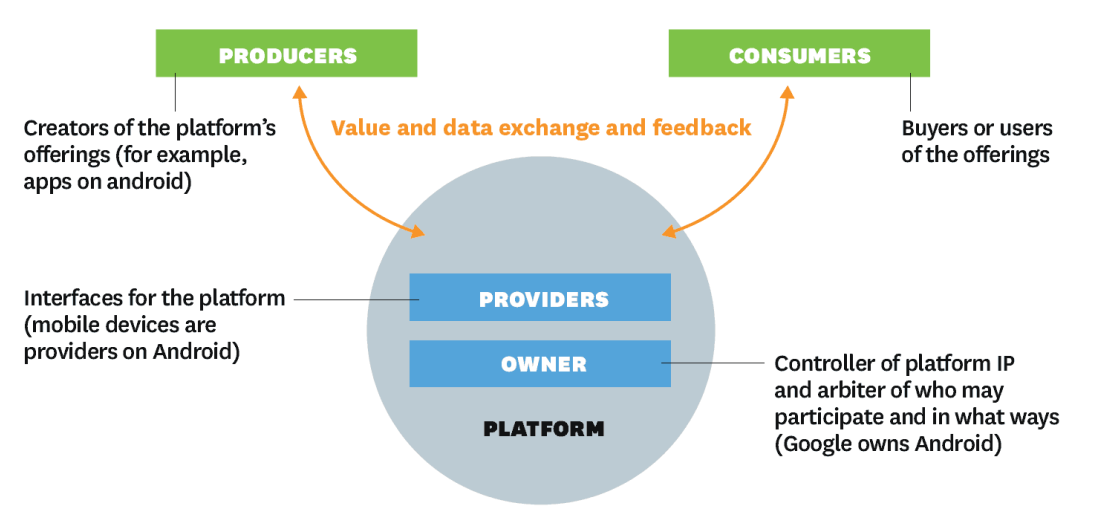
\includegraphics[scale=0.3]{image4.png}
Nel business delle piattaforme non ho un asset, quindi il mio valore non
deriva dagli asset bensì dagli utenti connessi e comunità che si sono
formate attorno a queste piattaforma. Questi modelli sono aperti e
permettono la partecipazione assistita e il vantaggio di queste imprese
deriva dal fatto che possono definire le proprie regole ed architetture.
Scalano molto rapidamente e si basano sugli effetti del network: Le
piattaforme sono in grado di far leva su questo effetto network, ovvero
l'economia di scala demand-side (dipende dal numero di utenti che usano
il servizio) e non sulla supply-side come nel modello tradizionale.

Quando parliamo di effetto network abbiamo due categorie:

\begin{itemize}
	 
	\item
	Same-Side (Diretto) -- Dal produttore(consumatore) al
	produttore(consumatore), quindi il valore aumenta o decresce se
	aumentano il numero di utenti dallo stesso lato (es. WhatsApp)
	\item
	Cross-Side (Indiretto) -- Dal produttore al consumatore (e viceversa),
	il valore aumenta se aumenta o decresce se aumenta o decresce la
	comunità di un lato rispetto all'altro (es. Trip Advisor, Uber)
\end{itemize}

Possono essere entrambi sia positivi che negativi come mostra i prossimi
schema:

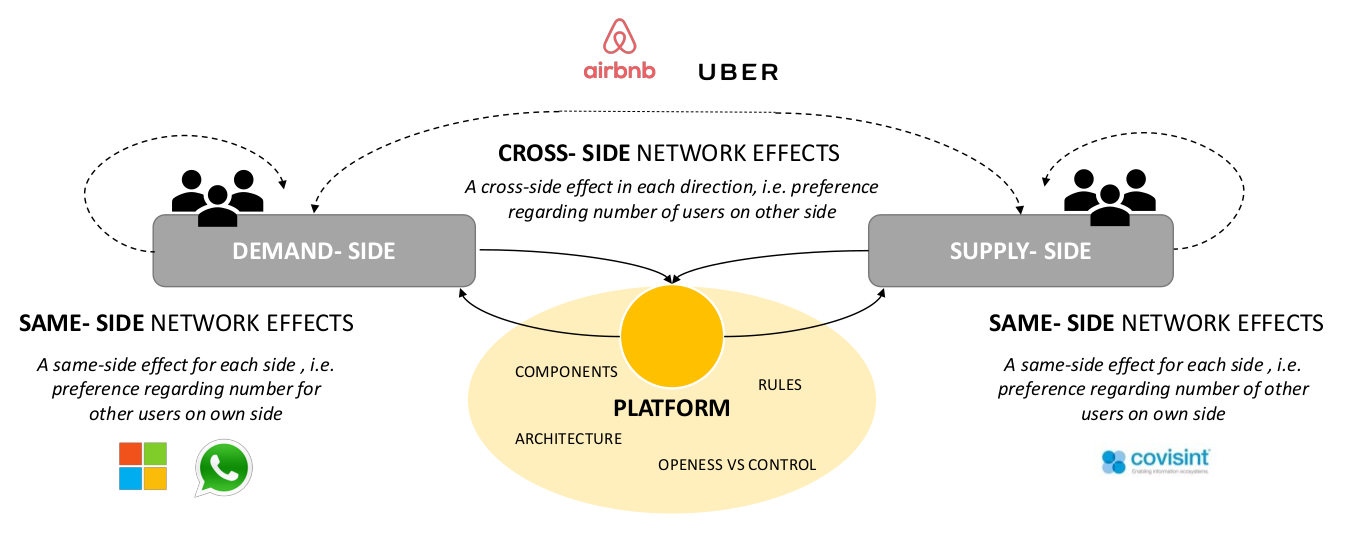
\includegraphics[scale=0.25]{image5.png}
Gli effetti positivi e negativi: \newline
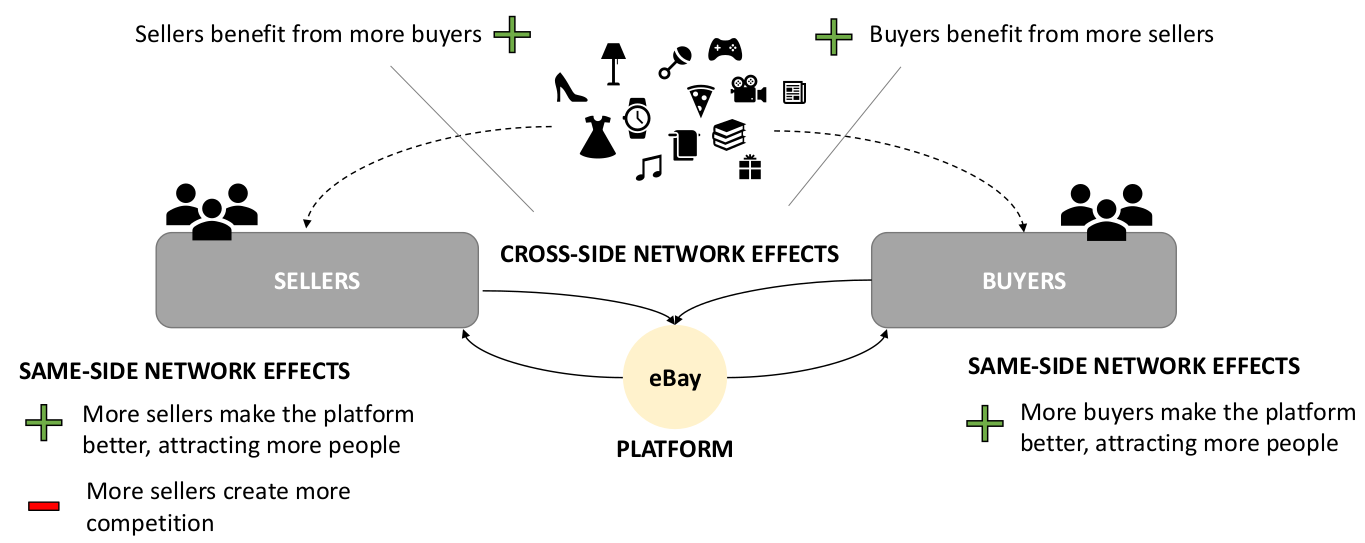
\includegraphics[scale=0.25]{image6.png}


Il fatto cruciale che permette il successo a questi modelli è
l'architettura. La chiave principale della architettura è la modularità:
un sistema che è diviso in un insieme di unità funzionanti, che
compongono una applicazione più grande.

Quindi una piattaforma, in termini di architetture, fatta di 3 elementi:

\begin{itemize}
	 
	\item
	Un insieme di componenti principali con un design stabile.
	\item
	Un insieme di componenti complementari.
	\item
	Un insieme di interfacce fisse che permettono inter-operabilità.
\end{itemize}

La modularità permette l'evoluzione e generazione di un ecosistema
digitale.

Un altro punto fondamentale è il trade-off tra apertura e il controllo
su tali sistemi, troppa apertura può portare alla frammentazione e
perdita di valore mentre troppo controllo può inibire l'innovazione,
quindi gli owner delle piattaforme devono applicare un sistema di cura
adeguato.

Questo trade-off tra controllo e generatività può essere espressa
attraverso governace delle piattaforme, 4 punti fondamentali di questa
governance sono:

\begin{itemize}
	 
	\item
	La legge
	\item
	Le norme
	\item
	L'architettura
	\item
	Il mercato
\end{itemize}

Anche self-governance è molto importante (e spesso efficace) per le
piattaforme. Sono ancora pochi i settori dell'economia rivoluzionati da
queste piattaforme, che hanno un potenziale altissimo. Più e più settori
si stanno avvicinando a questo approccio, questi settori sono
solitamente piene di informazioni, molto frammentate e hanno un
asimmetria informazionale estrema, mentre i settori che sono
pesantemente regolate e hanno un costo di fallimento molto alto non
verranno modificati tantissimo da questo modello delle piattaforme.

L'informazione è costosa da produrre ma quasi senza costo la sua
riproduzione, e il costo fisso della produzione è un sunk cost e non è
recuperabile una vota fermata la produzione. Il valore dell'informazione
è basato sul consumatore e non al suo costo di produzione, ma le persone
valorizzano l'informazione in maniera diversa e qui abbiamo il modello
differenziato del mercato del prodotto. Esistono tre tipi di
differential pricing:

\begin{itemize}
	 
	\item
	Personalized Pricing: Valuto l'informazione ottimizzato in base a
	ciascun cliente
	\item
	Versioning: Offro una linea prodotto e lascio l'utente decidere la
	versione per loro più appropriata.
	\item
	Group Pricing: Imposto prezzo diversificato per gruppi di consumatori,
	es. per studenti.
\end{itemize}

Un bene esperienzale è un bene che deve essere consumato/visto
dall'utente per valorizzarlo ad esempio un film, la maggior parte dei
nuovi prodotti sono beni esperienzali, ma l'informazione lo è ogni volta
che viene consumato. Per un cliente comprare informazioni prima di
sapere cosa siano può essere un problema, le diverse strategie adottate
sono: Avere anteprima delle informazioni e la marca/reputazione della
sorgente. Questo problema rimane uno dei problemi più grossi
dell'Information Age. Inoltre il problema non rimane più l'accesso
all'informazione bensì il suo sovraccarico. L'interfaccia che permette
di salvare, cercare, recuperare, copiare, filtrare, manipolare, vedere,
trasmettere e ricevere l'informazione è la tecnologia.
\addcontentsline{toc}{section}{Lezione Batini}
\section*{Lezione Batini -- 21/11}

I dato deriva dal latino datum, ciò che è stato dato, i dati
rappresentano il mondo che è passato almeno storicamente.

Partiamo dalle definizioni di dato, informazione e conoscenza:

\begin{itemize}
	 
	\item
	Dato: è il concetto meno astratto, seguito dall'informazione e infine
	la conoscenza è il concetto più astratto tra i tre. 
\end{itemize}

Ad esempio con la misuriamo la temperatura con un termometro che ci
segna 37.5, esso è un dato, il dato è una codifica grezza del mondo, e
da questo posso trarre delle informazioni, ma trarre informazioni
dipende dalla conoscenza che abbiamo. Quindi abbiamo che il dato 37.5
diventa informazione se noi sappiamo cos'è la temperatura (corporea) e
come si misura e in questo caso abbiamo l'informazione che è : ``La
temperatura corporea è pari a 37.5 $^o$C'' e da qui con la conoscenza
pregressa possiamo concludere di avere una febbre leggera.

La produzione dei dati, in generale, è una produzione che avviene
osservando la realtà e attraverso un processo di rappresentazione
(complesso) produrre attraverso quest'osservazione un
risultato/rappresentazione che può essere diversa in base al soggetto
che la rappresenta e/o l'obbiettivo di tale osservazione.

Il passaggio dai piccoli dati ai Big Data avviene principalmente in 3
direzioni:

\begin{itemize}
	 
	\item
	La prima è l'ampiezza della realtà osservata: ad esempio grazie ai
	satelliti possiamo vedere le cose da molto più in alto con molta più
	precisione
	\item
	La profondità nella conoscenza della realtà osservata: ad esempio i
	sensori nelle ruote di una macchina che li rendono ``intelligenti''.
	\item
	Il tempo: Possiamo studiare l'evoluzione nel tempo di tante cose con
	scale completamente diverse, ad esempio Il progresso di una città in
	mesi, oppure lo spostamento dei voli in secondi.
\end{itemize}

Le 5 grandi tecnologie che alimentano il mondo dei Big Data:

Possiamo vedere la dipendenza di queste varie tecnologia tra di loro.

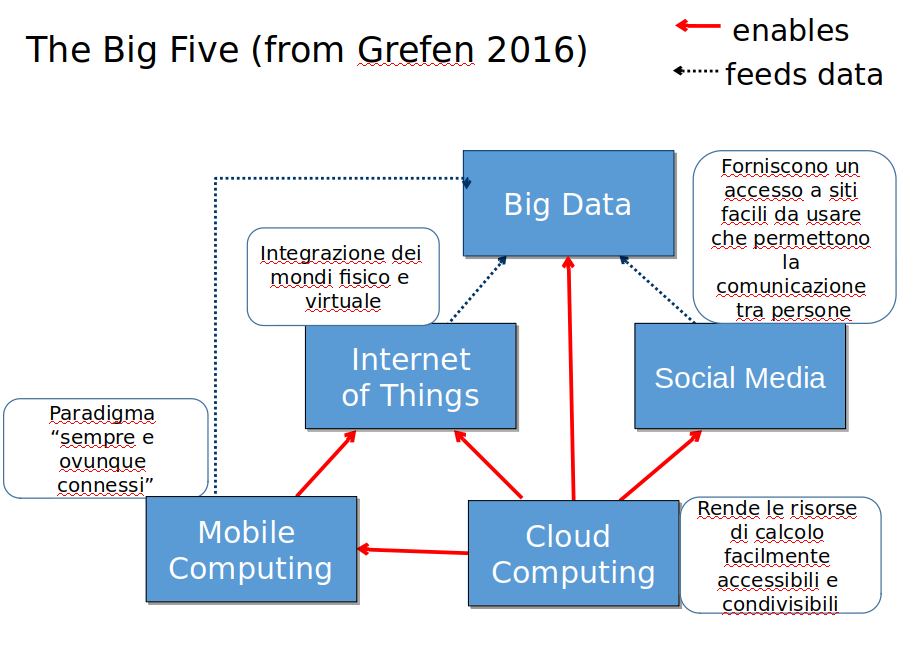
\includegraphics[scale=0.4]{image7.png}
Il ciclo di vita dell'informazione:

\begin{itemize}
	\item
	Formulazione del problema: devo capire a cosa mi possono servire i
	dati.
	\item
	Scelta delle fonti
	\item
	Gestione (o preparazione)
	
	\begin{itemize}
		 
		\item
		Valutazione e miglioramento della qualità
		\item
		Trasformazione
		\item
		Arricchimento semantico
		\item
		Integrazione
		\item
		Eliminazione dei dati non rivelanti
	\end{itemize}
	\item
	Visualizzazione esplorativa
	\item
	Analisi
	
	\begin{itemize}
		 
		\item
		Statistica classica
		\item
		Machine Learning
		\item
		Validazione della tecnica
	\end{itemize}
	\item
	Visualizzazione dei risultati
\end{itemize}

Secondo il World Economic Forum nel 2013, tra le minacce più grandi per
l'umanità si sono aggiunti: incidente massivo di frodi/furto dei dati,
cyberattacchi e disinformazione digitale massiva. E sempre più persone
usano le tecnologie che costano sempre di meno e si riesce a fare di
più. Ad esempio l'intelligenza usano aiuti dal computer per le analisi e
machine learning, che presto avranno una potenza migliore nel periodo a
venire. Le AI possono essere usate non solo per analizzare i dati ma
anche produrli (si veda il caso di nuove facce generate dal nvidia
oppure il giocatore di Go). E questo forgeria di AI presto sarà la causa
della scomparsa di fiducia sociale, poiché le prove prima affidabili
dopo non lo saranno più (un caso attuale è deepfake).

Il valore dei dati è un concetto molto ampio, ad esempio possiamo
scoprire gli evasori unendo i vari dati che abbiamo riguardo a una
persona (usando ML), che oggi sono molto separati. Un altro esempio è
prevedere i livelli di inquinamento, una start-up israeliana, di nome
BreezoMeter, produce delle heatmap e da qui c'è la possibilità di
prevedere, quest'applicazione è una combinazione e integrazione di
diversi fonti di dati e ipotesi, il che non è un processo triviale.

Il valore sociale dei dati: Il mondo digitale e analogico si stanno
incrociando sempre di più le macchine stanno sostituendo gli umani, ecc.
Questa sostituzione dell'uomo non è simmetrica nel senso che perché le
masse essendo molto grandi, necessariamente vengono trattate le
procedure automatiche. L'automatizzazione è rivolta sostanzialmente ai
numeri più grandi, e quelli che sfruttano queste masse sono i
privilegiati. Un esempio del valore sociale dei dati e l'Uganda dove i
dati riguardanti la health-care sono stati diffusi e questo ha portato a
un diminuzione della mortalità dei bambini con meno di 5 anni di un
terzo, solo la trasmissioni dei dati e nessun altro aiuto.

\end{document}
